\documentclass[11pt]{elegantbook}

\title{An Elegant \LaTeX{} Template for Books}
\subtitle{Classic Elegant\LaTeX{} Template}

\author{Ethan Deng \& Liam Huang}
\institute{Elegant\LaTeX{} Program}
\date{April 9, 2022}
\version{4.3}
\bioinfo{Bio}{Information}

\extrainfo{Victory won\rq t come to us unless we go to it. }

\logo{logo-blue.png}
\cover{cover.jpg}

% modify the color in the middle of titlepage
\definecolor{customcolor}{RGB}{32,178,170}
\colorlet{coverlinecolor}{customcolor}

\begin{document}

\maketitle

\frontmatter
\tableofcontents

\mainmatter

\chapter{Elegant\LaTeX{} Templates}
Elegant\LaTeX{} Program developers are intended to provide you beautiful, elegant, user-friendly templates. Currently, the Elegant\LaTeX{} is composed of \href{https://github.com/ElegantLaTeX/ElegantNote}{ElegantNote}, \href{https://github.com/ElegantLaTeX/ElegantBook}{ElegantBook}, \href{https://github.com/ElegantLaTeX/ElegantPaper}{ElegantPaper}, designed for typesetting notes, books, and working papers respectively. Latest releases are strongly recommended! This guide is aimed at briefly introducing the 101 of this template. For any other question, suggestion or comment, feel free to contact us on GitHub \href{https://github.com/ElegantLaTeX/ElegantBook/issues}{issues} or email us at \email{elegantlatex2e@gmail.com}.

Contact Infos:
\begin{itemize}
  \item GitHub: \href{https://github.com/ElegantLaTeX/}{https://github.com/ElegantLaTeX/}
  \item CTAN: \href{https://ctan.org/pkg/elegantbook}{https://ctan.org/pkg/elegantbook}
  \item Download: \href{https://github.com/ElegantLaTeX/ElegantBook/releases}{release}, \href{https://github.com/ElegantLaTeX/ElegantBook/archive/master.zip}{latest version}
\end{itemize}


\section{Online Usage}
You can visit \href{https://www.overleaf.com/}{Overleaf} to use our template online anywhere and anytime without local installation. To find our template, search \lstinline{elegantlatex} in the \lstinline{templates} or simply visit \href{https://www.overleaf.com/latex/templates?addsearch=elegantlatex}{search result}, choose the template you prefer and \lstinline{Open as Template} to own a copy yourself to edit freely. To learn more about Overleaf, please refer to \href{https://www.overleaf.com/learn}{Documentation}.


\section{Portable Version}
For portable version, simply download lastest ElegantBook-master from GitHub or CTAN (to be more accurate, download \lstinline{elegantbook.cls}) and save the file(s) under your working directory. This way of installation is simple and convenient, but you have to manually update \lstinline{cls} now and then.


\section{Update Templates}
You can use cmd/terminal to update the tlmgr itself and all the packages, the commands are:
\begin{lstlisting}
tlmgr update --self
tlmgr update --all
\end{lstlisting}

To learn more, please refer to \href{https://tex.stackexchange.com/questions/55437/how-do-i-update-my-tex-distribution}{How do I update my \TeX{} distribution?}

\section{Other Release Versions}
If you are a \TeX{} Live 2018/2019/2020/2021 user and would like to update, the official solution is to uninstall the previous version. If you want to save the bother of uninstallation and re-installation, please copy \lstinline{elegantbook.cls} to the installation directory of \TeX{} Live 2022 (default: \lstinline|C:\texlive\2022\texmf-dist\tex\latex\elegantbook| ), run \lstinline{texhash} in cmd.

\chapter{ElegantBook Settings}
This template is based on the Standard \LaTeX{} book class, so the options of book class work as well (Note that the option of papersize has no effect due to \lstinline{device} option). The default encoding is UTF-8 while \TeX{} Live is recommended. The test environment is Win10/Ubuntu 20.04/macOS + \TeX{} Live 2022/ Mac\TeX{} 2022, either \hologo{pdfLaTeX} or \hologo{XeLaTeX} works fine.

\section{Languages}
We defined one option named \lstinline{lang} which has two basic values, \lstinline{lang=en} (default) , \lstinline{lang=cn}. Different values will alter the captions of figure/table, abstract name, refname, etc. You can use this option as

\begin{lstlisting}
\documentclass[en]{elegantbook} 
\documentclass[lang=en]{elegantbook}
\end{lstlisting}

Besides the two basic language translation, our user provide more options, here is a short brief introduction to these translation. Since I am not familiar with these languages, I can't guarantee that the translations are correct, please comment on GitHub if you have some questions.

\begin{itemize}
  \item Italian translation \lstinline{lang=it}, provided by \href{https://github.com/VincentMVV}{VincentMVV} , please refer to \href{https://github.com/ElegantLaTeX/ElegantBook/issues/85}{Italian translation};
  \item French translation \lstinline{lang=fr}, provided by \href{https://github.com/abfek66}{abfek66} , please refer to \href{https://github.com/ElegantLaTeX/ElegantBook/issues/85}{Italian translation};
  \item Dutch Translation \lstinline{lang=nl}, provided by \href{https://github.com/inktvis75}{inktvis75} , please refer to \href{https://github.com/ElegantLaTeX/ElegantBook/issues/108}{Dutch Translation};
  \item Hungarian translation \lstinline{lang=hu}, provided by \href{https://github.com/palkotamas}{palkotamas}, please refer to \href{https://github.com/ElegantLaTeX/ElegantBook/issues/111}{Hungarian translation};
  \item Deutsch translation \lstinline{lang=de}, provided by Lisa, please refer to \href{https://github.com/ElegantLaTeX/ElegantBook/issues/113}{Deutsch translation};
  \item Spanish translation \lstinline{lang=es}, provided by Gustavo A. Corradi, please refer to \href{https://github.com/ElegantLaTeX/ElegantBook/issues/133}{Spanish translation};
  \item Mongolian translation \lstinline{lang=mn}, provided by \href{https://github.com/Altantsooj}{Altantsooj}, please refer to \href{https://github.com/ElegantLaTeX/ElegantBook/issues/137}{Mongolian translation};
  \item Japanese translation \lstinline{lang=jp}, provided by \href{https://github.com/inusturbo}{inusturbo}, please refer to \href{https://github.com/ElegantLaTeX/ElegantBook/issues/172}{Japanese translation}.
\end{itemize}

\begin{remark}
Chinese Characters  are acceptable \textbf{ONLY} in \lstinline{lang=cn}.
\end{remark}

\section{Device Mode Option}
The option for device (\lstinline{device}) was originally used in ElegantNote, now we include this option in ElegantBook\footnote{Pictures have to be modified accordingly.} as well. Activate iPad mode in the following way\footnote{Default size: normal, A4 paper.}:
\begin{lstlisting}
\documentclass[pad]{elegantbook} %or
\documentclass[device=pad]{elegantbook}
\end{lstlisting}

\section{Color Themes}
This template contains 5 color themes, i.e. \textcolor{structure1}{\lstinline{green}}\footnote{Original default theme.}, \textcolor{structure2}{\lstinline{cyan}}, \textcolor{structure3}{\lstinline{blue}}(default), \textcolor{structure4}{\lstinline{gray}}, \textcolor{structure5}{\lstinline{black}}. You can choose \lstinline{green} with
\begin{lstlisting}
\documentclass[green]{elegantbook} %or
\documentclass[color=green]{elegantbook}
\end{lstlisting}


\begin{table}[htbp]
\caption{ElegantBook Themes\label{tab:color thm}}
\centering
\begin{tabular}{ccccccc}
\toprule
          & \textcolor{structure1}{green} 
          & \textcolor{structure2}{cyan} 
          & \textcolor{structure3}{blue}
          & \textcolor{structure4}{gray} 
          & \textcolor{structure5}{black} 
          & Main Environments\\
\midrule
structure & \makecell{{\color{structure1}\rule{1cm}{1cm}}}
        & \makecell{{\color{structure2}\rule{1cm}{1cm}}}
        & \makecell{{\color{structure3}\rule{1cm}{1cm}}} 
        & \makecell{{\color{structure4}\rule{1cm}{1cm}}} 
        & \makecell{{\color{structure5}\rule{1cm}{1cm}}} 
        & chapter  section  subsection \\
main      & \makecell{{\color{main1}\rule{1cm}{1cm}}}
        & \makecell{{\color{main2}\rule{1cm}{1cm}}}
        & \makecell{{\color{main3}\rule{1cm}{1cm}}}
        & \makecell{{\color{main4}\rule{1cm}{1cm}}}
        & \makecell{{\color{main5}\rule{1cm}{1cm}}}
        & definition  exercise  problem  \\
second    & \makecell{{\color{second1}\rule{1cm}{1cm}}}
        & \makecell{{\color{second2}\rule{1cm}{1cm}}}
        & \makecell{{\color{second3}\rule{1cm}{1cm}}}
        & \makecell{{\color{second4}\rule{1cm}{1cm}}}
        & \makecell{{\color{second5}\rule{1cm}{1cm}}}
        & theorem  lemma  corollary\\
third     & \makecell{{\color{third1}\rule{1cm}{1cm}}}
        & \makecell{{\color{third2}\rule{1cm}{1cm}}}
        & \makecell{{\color{third3}\rule{1cm}{1cm}}}
        & \makecell{{\color{third4}\rule{1cm}{1cm}}}
        & \makecell{{\color{third5}\rule{1cm}{1cm}}}
        & proposition\\
\bottomrule
\end{tabular}
\end{table}

If you want to customize the colors, please select \lstinline{nocolor} or use \lstinline{color=none} and declare the main, second, and third colors in the preamble section as follows:
\begin{lstlisting}[frame=single]
\definecolor{structurecolor}{RGB}{60,113,183}
\definecolor{main}{RGB}{0,166,82}%
\definecolor{second}{RGB}{255,134,24}%
\definecolor{third}{RGB}{0,174,247}% 
\end{lstlisting}

\section{Cover}
\subsection{Customized Cover}
From v3.10, customized cover is allowed, you can choose or hide any element as you prefer. Current optional elements are:
\begin{itemize}
  \item title: \lstinline{\title}
  \item subtitle: \lstinline{\subtitle}
  \item author: \lstinline{\author}
  \item institute: \lstinline{\institute}
  \item date: \lstinline{\date}
  \item version: \lstinline{\version}
  \item extra information: \lstinline{\extrainfo}
  \item cover image: \lstinline{\cover}
  \item logo: \lstinline{\logo}
\end{itemize}

Besides, an extra command \lstinline{\bioinfo} is provided with two options--caption and content. For instance, if you want to display \lstinline{Username: 111520}, just type in

\begin{lstlisting}
\bioinfo{Username}{115520}
\end{lstlisting}

You can change the color of the horizontal bar of the cover by
\begin{lstlisting}
  \definecolor{customcolor}{RGB}{32,178,170}
  \colorlet{coverlinecolor}{customcolor}
\end{lstlisting}

\subsection{Cover Image}
The cover image used in this template is from \href{https://pixabay.com/en/tea-time-poetry-coffee-reading-3240766/}{pixabay.com}. The image is completely free and can be used under any circumstance. The cover image size is $1280 \times 1024$. If you would like to change the cover, please crop it according to the size of the cover picture strictly. One free online image clipping site: \href{https://www.fotor.com/cn}{fotor.com}. Feel free to join our QQ Group to get more elegant covers.

\subsection{Logo}
Aspect ratio of the logo is 1:1 in this guide, i.e. a square picture. To replace the logo, do remember to choose the appropriate picture.

\subsection{Stylized Cover}
Want to use stylized cover?(For instance, A4-sized PDF designed by Adobe Illustrator) Please comment out \lstinline{\maketitle} and use \lstinline{pdfpages} to insert the cover. Similar for using \lstinline{titlepage}. If you would like to use the cover in version 2.x, please refer to \href{https://github.com/EthanDeng/etitlepage}{etitlepage}.

\section{Chapter Title Display Styles}

This template contains 2 sets of \textit{title display styles},\lstinline{hang}(default) and \lstinline{display} style. For the former, chapter title is displayed on a single line (\lstinline{hang}). For the latter, chapter title is displayed on a double line (\lstinline{display}).In this guide, we use \lstinline{hang} . To change display style, use:
\begin{lstlisting}
\documentclass[hang]{elegantbook} %or
\documentclass[titlestyle=hang]{elegantbook}
\end{lstlisting}


\section{Introduction of Math Environments}
We defined two sets of theorem modes, \lstinline{simple} style and \lstinline{fancy} style (default). You may change to \lstinline{simple} mode by

\begin{lstlisting}
\documentclass[simple]{elegantbook} %or
\documentclass[mode=simple]{elegantbook}
\end{lstlisting}

In this template, we defined four different theorem class environments

\begin{itemize}
\item \textit{Theorem Environments}, including title and content, numbering corresponding to chapter. Three types depending on the format:
   \begin{itemize}
      \item \textcolor{main}{\textbf{definition}} environment, the color is  \textcolor{main}{main};
      \item \textcolor{second}{\textbf{theorem, lemma, corollary, axiom, postulate}} environment, the color is \textcolor{second} {second};
      \item \textcolor{third}{\textbf{proposition}} environment, the color is \textcolor{third}{third}.
   \end{itemize}
\item \textit{Example Environment}, including \textbf{example, exercise, problem} environment, auto numbering according to chapter.
\item \textit{Proof Environment}, including \textbf{proof, note} environment containing introductory symbol (\textbf{note} environment) or ending symbol (\textbf{proof} environment).
\item \textit{Conclusion Environment}, including \textbf{conclusion, assumption, property, remark and solution}\footnote{We also define an option \lstinline{result}, which can hide the \lstinline{solution} and \lstinline{proof} environments. You can switch between \lstinline{result=answer} and \lstinline{result=noanswer}.} environments, all of which begin with boldfaced words, with format consistent with normal paragraphs.
\end{itemize}

\subsection{Theorem Class Environments}
Since the template uses the \lstinline{tcolorbox} package to customize the theorem class environments, it is slightly different from the normal theorem environments. The usage is as follows:
\begin{lstlisting}
\begin{theorem}{theorem name}{label text}
The content of theorem.
\end{theorem}
\end{lstlisting}

The first parameter \lstinline{<theorem name>} represents the name of the theorem, and the second parameter \lstinline{label} represents the label used in cross-reference with \verb|ref{thm:label}|. Note that cross-references must be prefixed with \lstinline{thm:}. 

From version 4.1, you can write your theorem environments as follows:
\begin{lstlisting}
\begin{theorem}[theorem name]\label{thm:label text}
  The content of theorem.
\end{theorem}
% or
\begin{theorem}
  The content of theorem.
\end{theorem}
\end{lstlisting}

Other theorem class environments with the same usage includes:

\begin{table}[htbp]
  \centering
  \caption{Theorem Class Environments}
    \begin{tabular}{llll}
    \toprule
    Environment & Label text & Prefix & Cross-reference \\
    \midrule
    definition & label & def   & \lstinline|\ref{def:label}| \\
    theorem & label & thm   & \lstinline|\ref{thm:label}| \\
    postulate & label & pos & \lstinline|\ref{pos:label}| \\
    axiom & label & axi & \lstinline|\ref{axi:label}|\\
    lemma & label & lem   & \lstinline|\ref{lem:label}| \\
    corrlary & label & cor   & \lstinline|\ref{cor:label}| \\
    proposition & label & pro   & \lstinline|\ref{pro:label}| \\
    \bottomrule
    \end{tabular}%
  \label{tab:theorem-class}%
 \end{table}%
 
\subsection{Counter for Theorem Environments}

You can use \lstinline{thmcnt} option to control the theorem counter/number display style for the theorem environments, the acceptable options are \lstinline{chapter} (default) and \lstinline{section}. 

\begin{lstlisting}
\documentclass[section]{elegantbook} % turn the Theorem 4.1 to Theorem 4.1.1 
\documentclass[thmcnt=section]{elegantbook}
\end{lstlisting}



\subsection{Other Customized Environments}
The other three math environments can be called directly since there are no additional option for them, e.g. \lstinline{example}:
\begin{lstlisting}
\begin{example}
This is the content of example environment.
\end{example}
\end{lstlisting}

The effect is as follows:

\begin{example}
This is the content of example environment.
\end{example}

These are all similar environments with slight differences lies in:

\begin{itemize}
   \item Example, exercise, problem environments number within chapter;
   \item Note begins with introductory symbol and proof ends with ending symbol;
   \item Conclusion and other environments are normal paragraph environments with boldfaced introductory words.
\end{itemize}


\section{List Environments}
This template uses \lstinline{tikz} to customize the list environments, with \lstinline{itemize} environment customized to the third depth and \lstinline{enumerate} environment customized to fourth depth. The effect is as follows\\[2ex]
\begin{minipage}[b]{0.49\textwidth}
\begin{itemize}
   \item first item of nesti;
   \item second item of nesti;
   \begin{itemize}
      \item first item of nestii;
      \item second item of nestii;
      \begin{itemize}
         \item first item of nestiii;
         \item second item of nestiii.
      \end{itemize}   
   \end{itemize}
\end{itemize}
\end{minipage}
\begin{minipage}[b]{0.49\textwidth}
\begin{enumerate}
   \item first item of nesti;
   \item second item of nesti;
   \begin{enumerate}
      \item first item of nestii;
      \item second item of nestii;
      \begin{enumerate}
         \item first item of nestiii;
         \item second item of nestiii.
      \end{enumerate}   
   \end{enumerate}
\end{enumerate}
\end{minipage}


\section{Fonts}
\textcolor{red}{\bfseries Alert} After v3.10, newtx is reset to cm, together with other two options, the \lstinline{math} font option offers:
\begin{enumerate}
  \item \lstinline{math=cm}(default), use \LaTeX{} default math font (recommended).
  \item \lstinline{math=newtx}, use \lstinline{newtxmath} math font (may bring about bugs).
  \item \lstinline{math=mtpro2}, use \lstinline{mtpro2} package to set math font.
\end{enumerate}

If you use \lstinline{newtx} fonts, type in:
\begin{lstlisting}
\documentclass[math=newtx]{elegantbook}
\end{lstlisting}

When you are using \lstinline{newtx}, please pay attention to the hyphens. For instance,
\begin{equation}
\int_{R^q} f(x,y) dy.\emph{of\kern0pt f}
\end{equation}

The corresponding code is: 
\begin{lstlisting}
\begin{equation}
  \int_{R^q} f(x,y) dy.\emph{of \kern0pt f}
\end{equation}
\end{lstlisting}

\subsection{Symbol Fonts}
Feedback from some 3.08 users claims that error occurs when using our templates with  \lstinline{yhmath}, \lstinline{esvect} and other packages.
\begin{lstlisting}
LaTeX Error:
Too many symbol fonts declared.
\end{lstlisting}

The reason is that the template redefines font for math so that no new math font is allowed to be added. To use \lstinline{yhmath} and/or \lstinline{esvect}, please locate \lstinline{yhmath} or \lstinline{esvect} in \lstinline{elegantbook.cls}, uncomment corresponding related code.

\begin{lstlisting}
%%% use yhmath pkg, uncomment following code
% \let\oldwidering\widering
% \let\widering\undefined
% \RequirePackage{yhmath}
% \let\widering\oldwidering

%%% use esvect pkg, uncomment following code
% \RequirePackage{esvect}
\end{lstlisting}

\section{Bibliography}

This template uses biblatex to generate the bibliography, the default citestyle and bibliography style are both \lstinline{numeric}. Let's take a glance at the citation effect. ~\cite{en1} use data from a major peer-to-peer lending \cite{en3} marketplace in China to study whether female and male investors evaluate loan performance differently \parencite{en2}. 

If you want to use biblatex, you must create a file named \lstinline{reference.bib}, add bib items (from Google Scholar, Mendeley, EndNote, and etc.) to \lstinline{reference.bib} file, then cite the bibkey in the \lstinline{tex} file. The biber will automatically generate the bibliography for the reference you cited.


To change the bibliography style, this version introduces two options: \lstinline{citestyle} and \lstinline{bibstyle}, please refer to \href{https://ctan.org/pkg/biblatex}{CTAN:biblatex} for more detail about these options. You can change your bibliography style as

\begin{lstlisting}
\documentclass[citestyle=numeric-comp, bibstyle=authoryear]{elegantbook} 
\end{lstlisting}

We also add the \lstinline{bibend} option to this template, you can choose \lstinline{biber} (default) or \lstinline{bibtex} as you like, \lstinline{biber} is recommended.

\begin{lstlisting}
\documentclass[bibtex]{elegantbook} % or
\documentclass[bibend=bibtex]{elegantbook}
\end{lstlisting}

\section{Preface}

If you want to add a preface before the first chapter with the number of chapter unchanged, please add the preface in the following way:
\begin{lstlisting}
\chapter*{Introduction}
\markboth{Introduction}{Introduction}
The content of introduction.
\end{lstlisting}

\section{Content Option and Depth}
Option for content \lstinline{toc}, you can  choose either one column(\lstinline{onecol}) or two columns(\lstinline{twocol}). For two columns:
\begin{lstlisting}
\documentclass[twocol]{elegantbook}
\documentclass[toc=twocol]{elegantbook}
\end{lstlisting}

Default content depth is 1, use to use \lstinline|\setcounter{tocdepth}{2}|.

\section{Introduction Environment}
We create a introduction environment to display the structure of chapter. The basic useage is as follows:
\begin{lstlisting}
\begin{introduction}
  \item Definition of Theorem
  \item Ask for help
  \item Optimization Problem
  \item Property of Cauchy Series
  \item Angle of Corner
\end{introduction}
\end{lstlisting}
And you will get:
\begin{introduction}
  \item Definition of Theorem
  \item Ask for help
  \item Optimization Problem
  \item Property of Cauchy Series
  \item Angle of Corner
\end{introduction}

You can change the title of this environment by modifying the optional argument of this environment:
\begin{lstlisting}
\begin{introduction}[Brief Introduction]
...
\end{introduction}
\end{lstlisting}

%\section{Problem Set}
The environment \lstinline{problemset} is used at the end of each chapter to display corresponding exercises. Just type in the following sentences:
\begin{lstlisting}
\begin{problemset}
  \item exercise 1
  \item exercise 2
  \item exercise 3
\end{problemset}
\end{lstlisting}
And you will get:
\begin{problemset}
  \item exercise 1
  \item exercise 2
  \item exercise 3
  \item math equation test:
  \begin{equation}
  a^2+b^2=c_{2_{i}} (1,2) [1,23]
  \end{equation}
\end{problemset}
\begin{remark}
If you want to customize the title of \lstinline{problemset}, please change the optional argument like in introduction environment. In this version the \lstinline{problemset} environment automatically appears in the table of contents but not in the header or footer(to be fixed).
\end{remark}

\begin{solution}
  If you want to customize the title of \lstinline{problemset}, please change the optional argument like in introduction environment. In this version the \lstinline{problemset} environment automatically appears in the table of contents but not in the header or footer(to be fixed).
\end{solution}

\section{Margin Notes}
In 3.08, we introduced \lstinline{marginpar=margintrue} and \lstinline{\elegantpar} (Beta) with piles of bugs. Hence we decide to remove them in 3.09 and will suspend the options till revolutionary optimization. Sorry for all the bugs! However, we retain the option \lstinline{marginpar} for users to get margin motes by activating \lstinline{marginpar=margintrue} and using \lstinline{\marginpar} or \lstinline{marginnote} packages.

\begin{remark}
Note that text and equation are both available in the margin notes.
\begin{lstlisting}
% text
\marginpar{margin paragraph text}

% equation
\marginpar{
\begin{equation}
  a^2 + b^2 = c^2
\end{equation}
}
\end{lstlisting}

For tables and figures, note that floating environment is not allowed. You have to use \lstinline{includegraphics} or \lstinline{table} and use \lstinline{\captionof} to name it. To get centralized figures or tables, use \lstinline{\centerline} or \lstinline{center}. To learn more, please refer to \href{https://tex.stackexchange.com/questions/5583/caption-of-figure-in-marginpar-and-caption-of-wrapfigure-in-margin}{Caption of Figure in Marginpar}.

\begin{lstlisting}
% graph with centerline command
\marginpar{
  \centerline{
    \includegraphics[width=0.2\textwidth]{logo.png}
  }
  \captionof{figure}{your figure caption}
}

% graph with center environment
\marginpar{
  \begin{center}
    \includegraphics[width=0.2\textwidth]{logo.png}
    \captionof{figure}{your figure caption}
  \end{center}
}
\end{lstlisting}

\end{remark}



\chapter{ElegantBook Writing Sample}

\begin{introduction}
\item Theorem Class Envrionments
\item Cross Reference
\item Math Environments
\item List Environments
\item Logo and Base 
\item $a^2+b^2=c^2$
\end{introduction}


\lipsum[1]
% source: https://www.maths.tcd.ie/~dwilkins/LaTeXPrimer/Theorems.html

\section{Writing Sample}

We will define the integral of a measurable function in three steps. First, we define the integral of a nonnegative simple function. Let $E$ be the measurable set in $\mathcal{R}^N$.

\begin{definition}[Left Coset]
Let $H$ be a subgroup of a group~$G$.  A \emph{left coset} of $H$ in $G$ is a subset of $G$ that is of the form $xH$, where $x \in G$ and $xH = \{ xh : h \in H \}$. Similarly a \emph{right coset} of $H$ in $G$ is a subset of $G$ that is of the form $Hx$, where $Hx = \{ hx : h \in H \} \hbar$ 
\end{definition}

\begin{note}
Note that a subgroup~$H$ of a group $G$ is itself a left coset of $H$ in $G$.
\end{note}

\lipsum[2]

\begin{theorem}[Lagrange's Theorem] \label{thm:lg}
Let $G$ be a finite group, and let $H$ be a subgroup of $G$. Then the order of $H$ divides the order of $G$.
\end{theorem}

As theorem \ref{thm:lg} refered.

\lipsum[3]


\begin{theorem}{theorem name}{label text}
  The content of theorem.
\end{theorem}

we can refer this theorem as \ref{thm:label text}.


\begin{proposition}[Size of Left Coset]
Let $H$ be a finite subgroup of a group $G$.  Then each left coset of $H$ in $G$ has the same number of elements as $H$.
\end{proposition}

\begin{proof}
  Let $z$ be some element of $xH \cap yH$. Then $z = xa$ for some $a \in H$, and $z = yb$ for some $b \in H$. If $h$ is any element of $H$ then $ah \in H$ and $a^{-1}h \in H$, since $H$ is a subgroup of $G$. But $zh = x(ah)$ and $xh = z(a^{-1}h)$ for all $h \in H$. Therefore $zH \subset xH$ and $xH \subset zH$, and thus $xH = zH$.  Similarly $yH = zH$, and thus $xH = yH$, as required. 
\end{proof}

\begin{figure}[htbp]
  \centering
  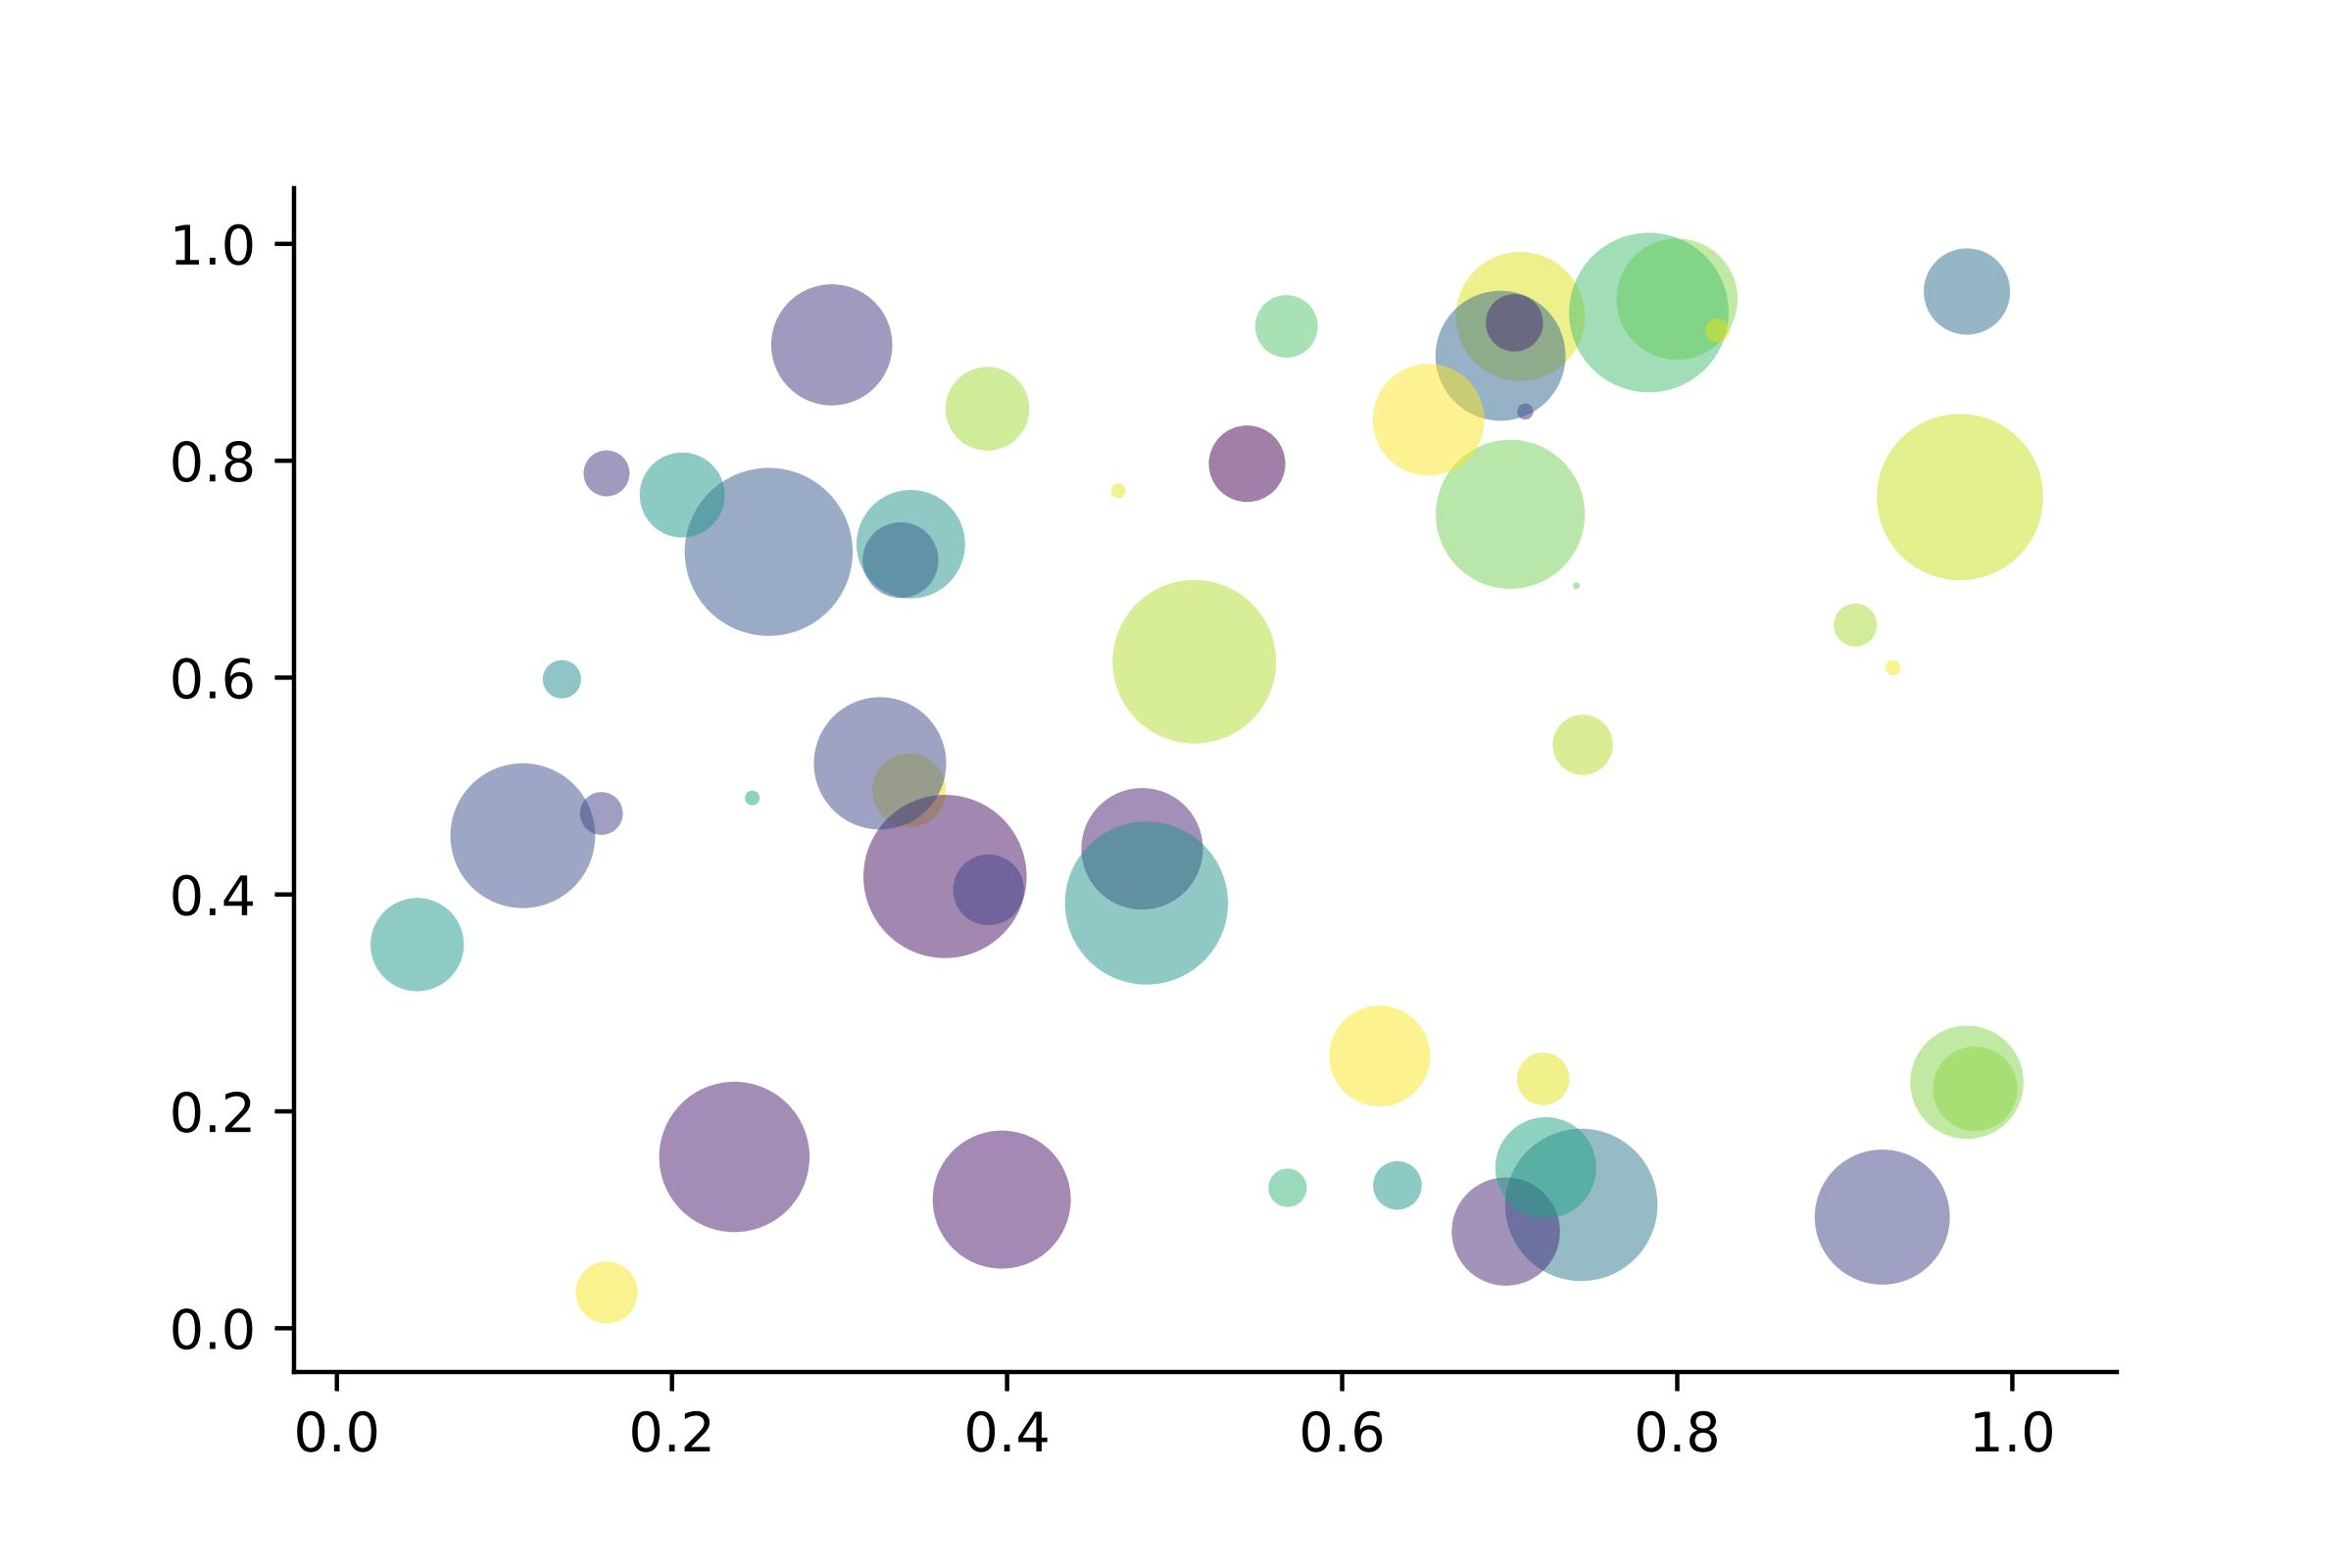
\includegraphics[width=0.6\textwidth]{scatter.jpg}
  \caption{Matplotlib: Scatter Plot Example\label{fig:scatter}}
\end{figure}

Regression analysis is a powerful statistical method that allows you to examine the relationship between two or more variables of interest. While there are many types of regression analysis, at their core they all examine the influence of one or more independent variables on a dependent variable. The process of performing a regression allows you to confidently determine which factors matter most, which factors can be ignored, and how these factors influence each other.

Let's continue using our application training example. In this case, we'd want to measure the historical levels of satisfaction with the events from the past three years or so, as well as any information possible in regards to the independent variables. 

\section{Second section}
This second section\index{S!section} may include some special word, 
and expand the ones already used\index{keywords!used}.


\begin{table}[htbp]
  \small
  \centering
  \caption{Auto MPG and Price \label{tab:reg}}
    \begin{tabular}{lcc}
    \toprule
                    &       (1)         &        (2)      \\
    \midrule
    mpg             &    -238.90***     &      -49.51     \\
                    &     (53.08)       &      (86.16)    \\
    weight          &                   &      1.75***    \\
                    &                   &      (0.641)    \\
    constant        &     11,253***     &       1,946     \\
                    &     (1,171)       &      (3,597)   \\
    obs             &        74         &         74     \\
    $R^2$           &      0.220        &       0.293    \\
    \bottomrule
    \multicolumn{3}{l}{\scriptsize Standard errors in parentheses} \\
    \multicolumn{3}{l}{\scriptsize *** p<0.01, ** p<0.05, * p<0.1} \\
    \end{tabular}%
\end{table}%

\lipsum[1-2]

\begin{itemize}
  \item Routing and resource discovery;
       \begin{itemize} 
             \item Language Models
            \item Vector Space Models
         \end{itemize}
  \item Resilient and scalable computer networks;
  \item Distributed storage and search.
\end{itemize}

%\problemset
\begin{problemset}
  \item Solve the equation $5(- 3x - 2) - (x - 3) = -4(4x + 5) + 13$.
  \item Find the distance between the points $(-4 , -5)$ and $(-1 , -1)$.
  \item Find the slope of the line $5x - 5y = 7$.
\end{problemset}


\chapter{FAQ}
We list some FAQs for users to refer to:
\begin{enumerate}
  \item \question{Why option numbers for natbib fail to take effect in v3.07?}
  In v3.07, when \lstinline{gbt7714} is introduced, option \lstinline{authoryear} is incompatible with \lstinline{natbib}. In v3.08 and 3.09, \lstinline{numbers}, \lstinline{numbers}, \lstinline{super} and \lstinline{authoryear} are introduced.
  \item \question{I want to customize font and background color.}
  Please use \lstinline{pagecolor} to change background color, refer to \href{https://tex.stackexchange.com/questions/278544/xcolor-what-is-the-equivalent-of-default-text-color}{this} to customize font.
  \item \question{Which version should I choose?}
  Please use \href{https://github.com/ElegantLaTeX/ElegantBook/releases}{Latest Release} via GitHub or \TeX{} Live 2022.
  \item \question{Which editor should I choose?}
  You can use \TeX{} Live 2022 built-in \TeX works or \TeX Studio. You may refer to \href{https://github.com/EthanDeng/texworks-autocomplete}{\TeX{}works autocomplete}. \TeX{} Live 2022 + \TeX{}studio is strongly recommended. Related configurations can be found at \href{https://github.com/EthanDeng/vscode-latex}{vscode-latex} and \href{https://github.com/EthanDeng/sublime-text-latex}{sublime-text-latex}.
  \item \question{Hello, we want to use ElegantBook to write a book about machine learning and would like your authorization.}
  Feel free to use our templates by pointing out our copyright. For other issues, please refer to LPPL-1.3c. If you want to show us your work, you can share the URL with us afterwards.
  \item \question{What is cross reference?}
  This template is aimed at who are not a complete beginner for \LaTeX{}. Please learn more about \LaTeX{} before using this template.
  \item \question{Is the language for code highlighting optional?}
  Yes, \lstinline{listings} package is used in ElegantBook, hence language is optional(e.g. \lstinline{language=Python}). For global setting, use \lstinline{lstset}. For more information, please refer to package documentations.
  \item \question{When will Beamer template (ElegantSlide or ElegantBeamer) forthcoming?}
  Since there is an excellent theme \href{https://github.com/matze/mtheme}{Metropolis}, no plan for Beamer theme.
\end{enumerate}

\chapter{Version History}
We revised our templates now and then. This section shows the version story of ElegantBook.


\datechange{2022/04/09}{release of v4.3.}

\begin{change}
  \item Remove part newtx settings, set TeX Gyre Terms/Heros fonts under \hologo{XeLaTeX}.
  \item Fix Chinese fonts in the theorem environments.
  \item Add theorem counter option, \lstinline{thmcnt=section}.
  \item Add bib option \lstinline{bibend}, which can take value of biber and bibtex.
  \item \textbf{! Warnings}: The multilingual option may cause some unexpected errors, you can report in this \href{https://github.com/ElegantLaTeX/ElegantBook/issues/170}{issue}.
\end{change}



\datechange{2022/03/08}{release of v4.2.}

\begin{change}
  \item Bug fix due to the update of newtx fonts;
  \item Add `Chapter' in TOC, and redefine \lstinline{\chaptername} to unify the logic under different languages;
  \item Add language option for Japanese, \lstinline{lang=jp}.
\end{change}


\datechange{2021/05/02}{release of v4.1.}

\begin{change}
  \item \textbf{! Big Change}: Change the bibliography method from \hologo{BibTeX} to biblatex(with backend  \lstinline{biber});
  \item \textbf{! Big Change}: Add support for the default theorem writing method (with optional name and label);
  \item Add left and right space;
  \item Support hyperlink from the text of TOC;
  \item Remove the \hologo{pdfLaTeX} compatiblity check for Chinese.
  \item Add multilingual support, for french \lstinline{lang=fr}, dutch \lstinline{lang=nl}, Hungarian  \lstinline{lang=hu}, Spanish \lstinline{lang=es}, Mongolian \lstinline{lang=mn} etc.
\end{change}

\datechange{2020/04/12}{release of v3.11, \textcolor{red}{\textbf{LAST} version of 3.x}.}


\begin{change}
  \item \textbf{! Fix}: Fix \lstinline{natbib option clash} problems caused by \lstinline{gbt7714} updates.
  \item Remove \lstinline{base} decorations and its options since \lstinline{pgfornament} package is not included in \TeX{} Live 2020.
  \item Fix spacing problem in some environments.
  \item Introduce language option for Italian, \lstinline{lang=it}.
\end{change}


\datechange{2020/02/10}{release of v3.10}

\begin{change}
  \item Introduce \lstinline{math} for math font, optional styles are \lstinline{newtx} and \lstinline{cm}.\\
  \textbf{Notice}: The math font \lstinline{newtxmath} in previous versions is reset to default \LaTeX{} math font, to keep previous math font, please declare \lstinline{math=newtx}.
  \item Introduce \lstinline{chinesefont} option, with \lstinline{founder}, \lstinline{ctexfont} and \lstinline{nofont} available.
  \item Turn author information on the cover optional and add customized command \lstinline{\bioinfo}.
  \item Add version history with command \lstinline{\datechange} and environment \lstinline{change}.
  \item Add Chinese chapter style \lstinline{scheme} with option \lstinline{chinese}.
  \item Since the bug raised by \lstinline{\lvert} is fixed, exchange package positions of \lstinline{ctex} and \lstinline{amsmath}.
  \item Drop \lstinline{\lastpage} from header to avoid page anchor bug and adding \lstinline{\frontmatter}.
  \item Revise bibliography option \lstinline{cite} with optional styles \lstinline{numbers},\lstinline{authoryear} and \lstinline{super}.
  \item Introduce bibliography style option \lstinline{bibstyle}, with default bib style \lstinline{apalike} for English mode and \lstinline{gbt7714} package for Chinese mode.
\end{change}

\datechange{2019/08/18}{release of v3.09}

\begin{change}
  \item Remove \lstinline{\elegantpar} temporary and remind users to use \lstinline{\marginnote} and \lstinline{\marginpar} instead.
  \item Use \lstinline{esint} to display integral operator.
  \item Add new command \lstinline{toc}, with options  \lstinline{onecol} and \lstinline{twocol}.
  \item Add new option \lstinline{cite} \lstinline{super} for superscript-displayed citation.
  \item Revise \lstinline{problemset}.
\end{change}

\nocite{en2,en3}

\printbibliography[heading=bibintoc, title=\ebibname]

\appendix
% \renewcommand\chaptername{\eappendix \thechapter}

\chapter{Mathematical Tools}

This appendix covers some of the basic mathematics used in econometrics. We briefly discuss the properties of summation operators, study the properties of linear and some nonlinear equations, and review the ratios and percentages. We also introduce some special functions that are common in econometrics applications, including quadratic functions and natural logarithms. The first four sections require only basic algebraic techniques. The fifth section briefly reviews differential Calculus Although Calculus is not necessary to understand much of this book, it is used in some of the end-of-chapter appendices and in some of the more advanced topics in part 3.

\section{Summation Operator and Description Statistics}

\textbf{Summation Operator} is an abbreviation used to express the summation of numbers, it plays an important role in statistics and econometrics analysis. If $\{x_i: i=1, 2, \ldots, n\}$ is a sequence of $n$ numbers, the summation of the $n$ numbers is:

\begin{equation}
\sum_{i=1}^n x_i \equiv x_1 + x_2 +\cdots + x_n
\end{equation}


\end{document}